%*----------- SLIDE -------------------------------------------------------------
\begin{frame}[t]{Contexto} 
    \transdissolve[duration=0.5]
    A pesquisa desta tese visa desenvolver um modelo para a compensação das perturbações sofridas por manipuladores utilizados em veículos submarinos remotamente controlados, buscando dessa forma uma maior eficiência no planejamento e realização de trajetórias específicas de atividades submarinas.\\
    \vspace*{0.2cm}
    Pontos cruciais para o setor de atividades submarinas utilizando veículos submarinos:
    \newline
        \begin{columns}[c]
            \column{.05\textwidth}
            \column{.35\textwidth}
                \begin{enumerate}
                    \item tempo de realização da atividade;
                    \item complexidade da operação;
                    \item eficiência da tarefa.
                \end{enumerate}
            \column{.6\textwidth}
            \includemedia[
                width=0.7\linewidth,
                totalheight=0.39375\linewidth,
                activate=pageopen,
                passcontext, 
                addresource=./Media/movies/rov-fixing.mp4,
                flashvars={
                source=./Media/movies/rov-fixing.mp4
                &autoPlay=true
                &Loop=false}
                ]{\fbox{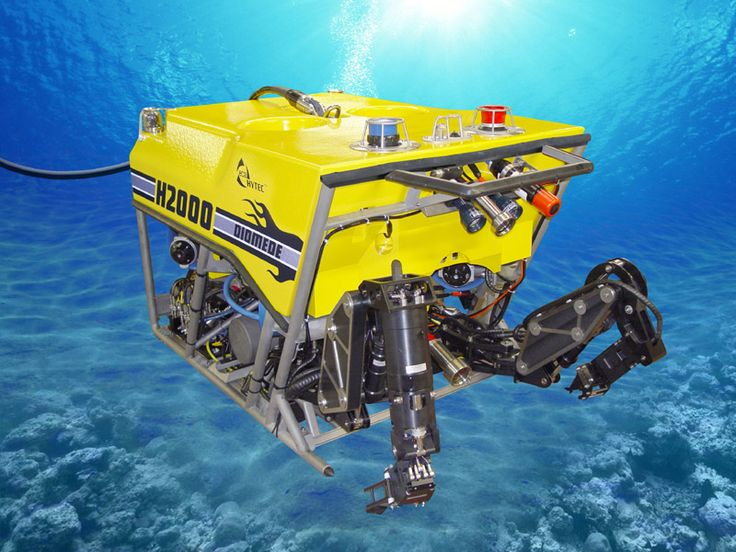
\includegraphics{rov}}}{VPlayer.swf}
        \end{columns}
%*----------- notes
    \note[item]{Notes can help you to remember important information. Turn on the notes option.}
\end{frame}
%-
\begin{frame}[c]{O Sistema}
    %\transboxin[duration=1,direction=30]

    \centering
    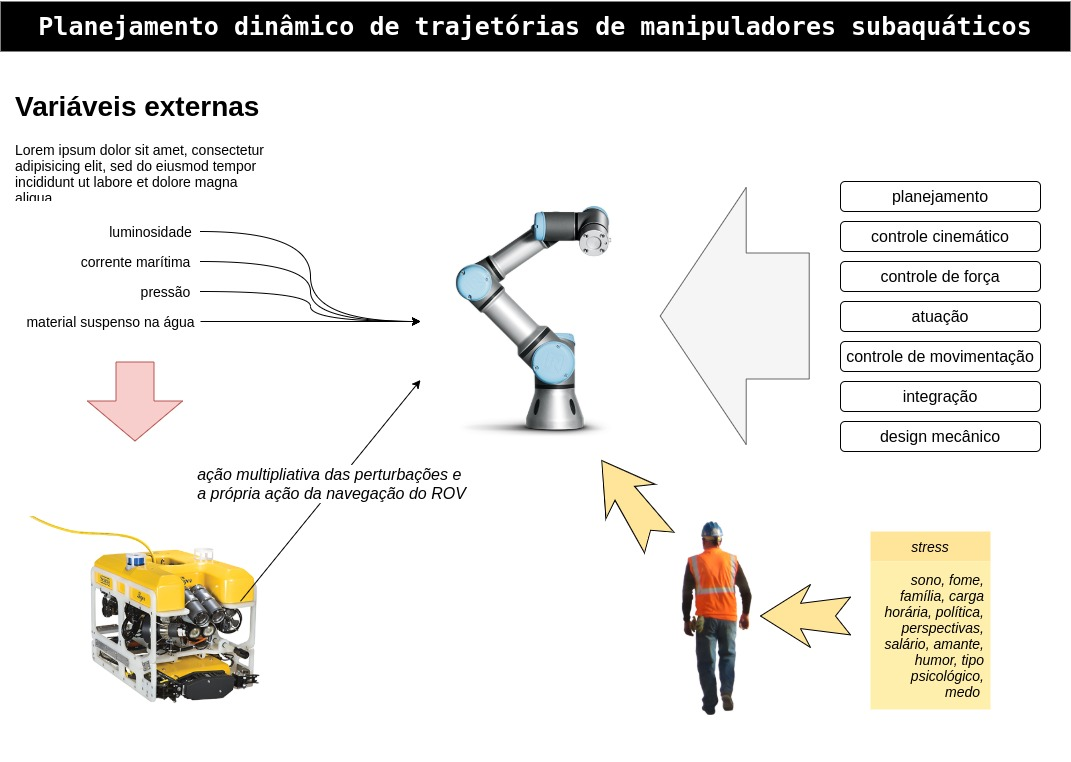
\includegraphics[width=.75\textwidth]{osistema}

    %\centering
    % \begin{columns}
    %     \column{.02\textwidth}
    %     \column{.48\textwidth}
    %     \begin{itemize}
    %         \item Planejamento dinâmico de trajetórias.
    %         \item Odometria visual.
    %         \item Manipuladores subaquáticos.
    %         \item Manipuladores autônomos.
    %         \item Manipuladores subaquáticos autônomos.
    %         \item Operação submarina autônoma.
    %     \end{itemize}
    %     \column{.25\textwidth}
    %         \centering
    %         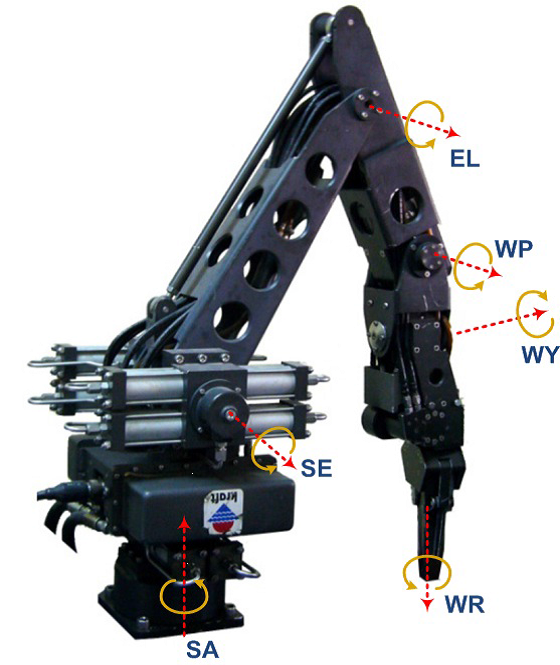
\includegraphics[width=1\textwidth]{kraft}\\
    %         
\includegraphics[width=.6\textwidth]{apriltag}
    %     \column{.25\textwidth}
    %         \centering
    %         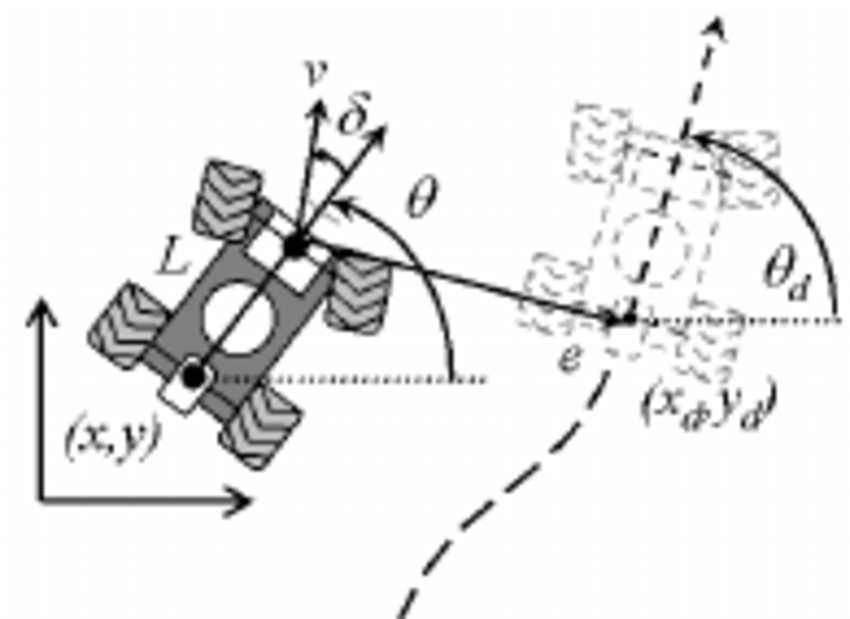
\includegraphics[width=1\textwidth]{visualodom}\\
    %         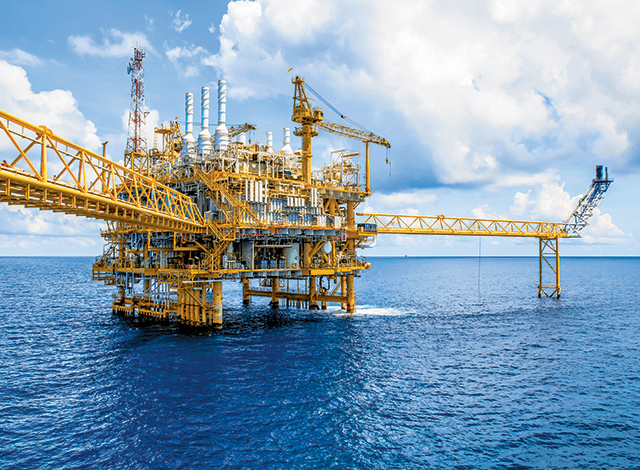
\includegraphics[width=1\textwidth]{opsub}

    %     % \begin{figure}[ht] \label{ fig7} 
    %     %     \begin{minipage}[b]{0.5\linewidth}
    %     %       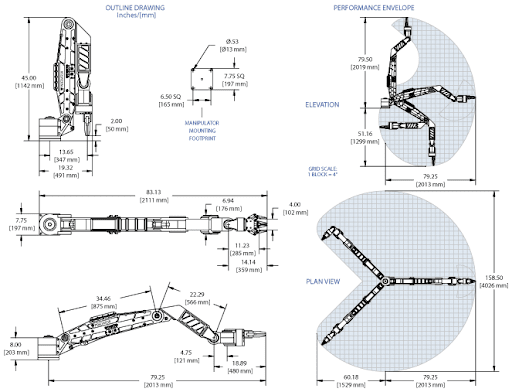
\includegraphics[width=.5\linewidth]{blueprint-arm} 
    %     %       \caption{Initial condition} 
    %     %     \end{minipage} 
    %     %     \begin{minipage}[b]{0.5\linewidth}
    %     %       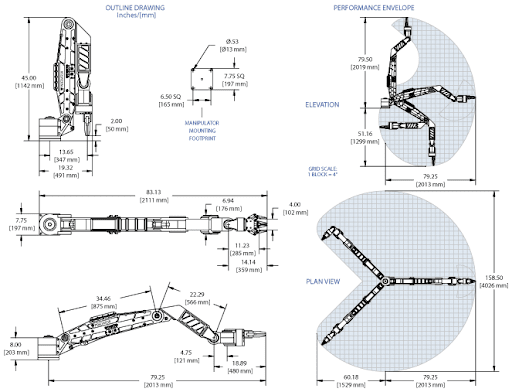
\includegraphics[width=.5\linewidth]{blueprint-arm} 
    %     %       \caption{Rupture} 
    %     %     \end{minipage} 
    %     %     \begin{minipage}[b]{0.5\linewidth}
    %     %       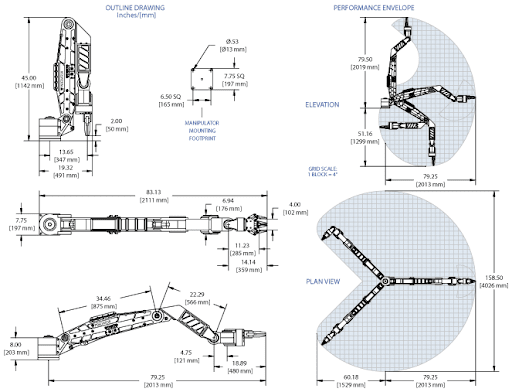
\includegraphics[width=.5\linewidth]{blueprint-arm} 
    %     %       \caption{DFT, Initial condition} 
    %     %     \end{minipage}
    %     %     \hfill
    %     %     \begin{minipage}[b]{0.5\linewidth}
    %     %       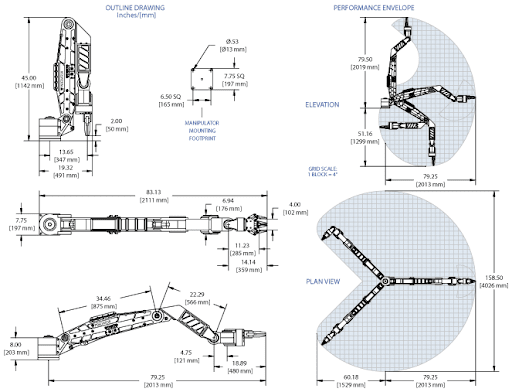
\includegraphics[width=.5\linewidth]{blueprint-arm} 
    %     %       \caption{DFT, rupture} 
    %     %     \end{minipage} 
    %     %   \end{figure}
    % \end{columns}
    % \begin{itemize}
    %     \item Planejamento de trajetórias.
    %     \item Odometria visual.
    %     \item Manipuladores subaquáticos.
    %     \item Manipuladores autônomos.
    %     \item Manipuladores subaquáticos autônomos.
    %     \item Operação submarina autônoma.
    % \end{itemize}
    % \begin{block}
    %     {MANIPULADOR}{manipulador}
    % \end{block}

%*----------- notes
    \note[item]{Notes can help you to remember important information. Turn on the notes option.}
\end{frame}
%-
%*----------- SLIDE -------------------------------------------------------------
\begin{frame}[c]{Questões de Pesquisa}
    \transboxout[duration=0.5]
    \begin{columns}
        \column{.05\textwidth}
        \column{.40\textwidth}
            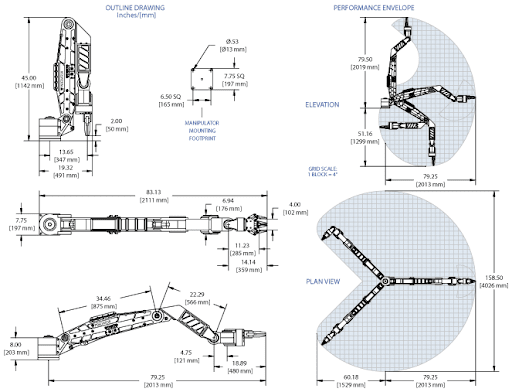
\includegraphics[width=1.1\textwidth]{blueprint-arm}
        \column{.55\textwidth}
            \begin{enumerate}
                \item De que forma as perturbações podem ser compensadas num manipulador submarino?
                \item Qual o modelo para uma melhor eficiência de trajetórias?
                \item Quais variáveis são preponderantes para um controle de trajetórias?
                \item Como estas variáveis podem interferir num novo modelo?
            \end{enumerate}
    \end{columns}
%*----------- notes
    \note[item]{Notes can help you to remember important information. Turn on the notes option.}
\end{frame}
%-
%*----------- SLIDE -------------------------------------------------------------
\begin{frame}[c]{Objetivo geral}
    %\transboxin[duration=1,direction=30]
    %\setbeamercolor{background canvas}{bg=yellow}
    \Wider{%
    \begin{shaded}
    \begin{center}
        \resizebox{!}{0.5cm}{%
            Propor um modelo dinâmico para
        }%
        \\
        \vspace*{0.5cm}
        \resizebox{!}{0.7cm}{%
            planejamento de trajetórias.
        }%
    \end{center}
    \end{shaded}
    }%
%*----------- notes
    \note[item]{Notes can help you to remember important information. Turn on the notes option.}
\end{frame}
%-
\begin{frame}[c]{Objetivos específicos}
    %\transboxin[duration=1,direction=30]
    \centering
    \begin{enumerate}
        \item Realizar \textbf{comparação} entre modelos existentes de planejamento de trajetórias.
        \item Implementar \textbf{odometria visual} num manipulador.
        \item \textbf{Integrar} a odometrial visual com o modelo de planejamento de trajetórias.
        \item \textbf{Simular o modelo} no sistema proposto do manipulador.
    \end{enumerate}
%*----------- notes
    \note[item]{Notes can help you to remember important information. Turn on the notes option.}
\end{frame}
%-
\begin{frame}[c]{Categorias Teóricas}
    %\transboxin[duration=1,direction=30]
    \centering
    \begin{columns}
        \column{.02\textwidth}
        \column{.48\textwidth}
        \begin{itemize}
            \item Planejamento dinâmico de trajetórias.
            \item Odometria visual.
            \item Manipuladores subaquáticos.
            \item Manipuladores autônomos.
            \item Manipuladores subaquáticos autônomos.
            \item Operação submarina autônoma.
        \end{itemize}
        \column{.25\textwidth}
            \centering
            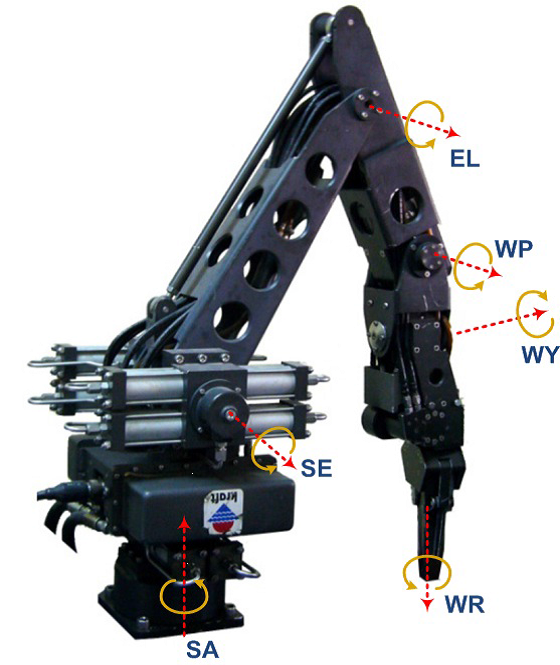
\includegraphics[width=1\textwidth]{kraft}\\
            
\includegraphics[width=.6\textwidth]{apriltag}
        \column{.25\textwidth}
            \centering
            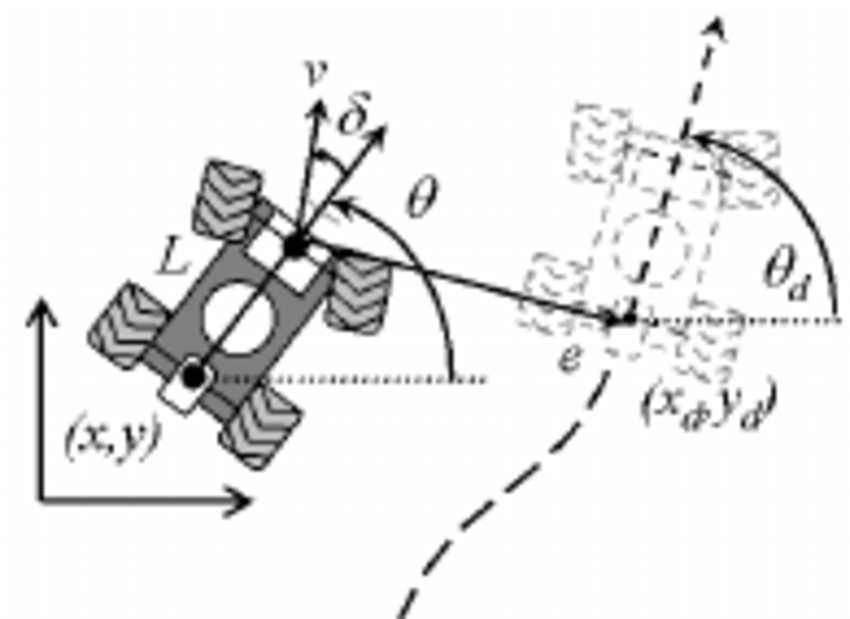
\includegraphics[width=1\textwidth]{visualodom}\\
            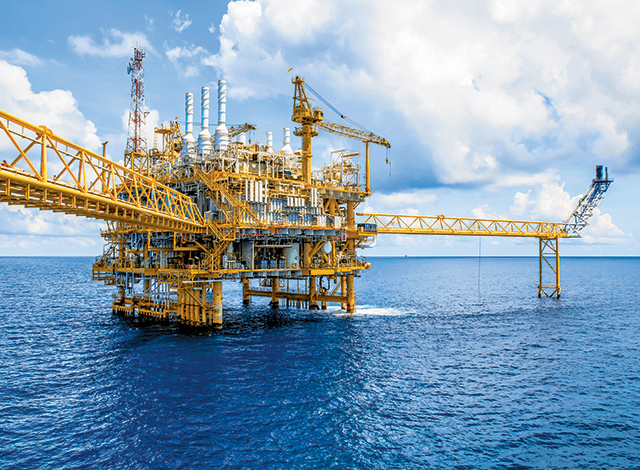
\includegraphics[width=1\textwidth]{opsub}

        % \begin{figure}[ht] \label{ fig7} 
        %     \begin{minipage}[b]{0.5\linewidth}
        %       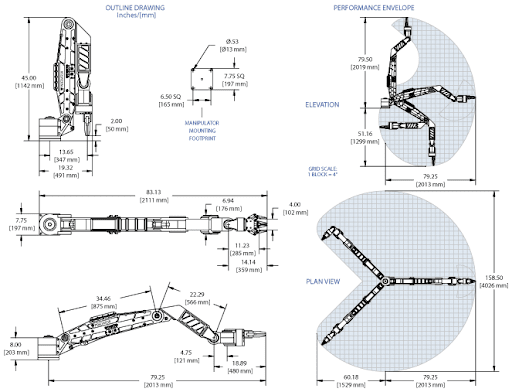
\includegraphics[width=.5\linewidth]{blueprint-arm} 
        %       \caption{Initial condition} 
        %     \end{minipage} 
        %     \begin{minipage}[b]{0.5\linewidth}
        %       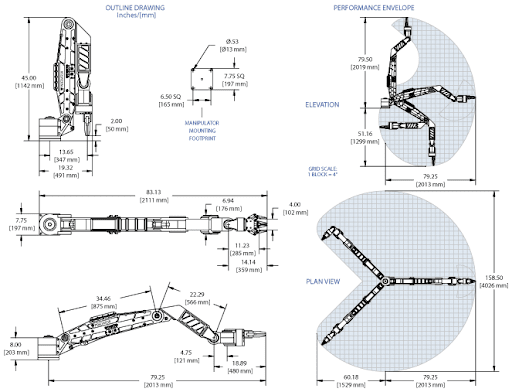
\includegraphics[width=.5\linewidth]{blueprint-arm} 
        %       \caption{Rupture} 
        %     \end{minipage} 
        %     \begin{minipage}[b]{0.5\linewidth}
        %       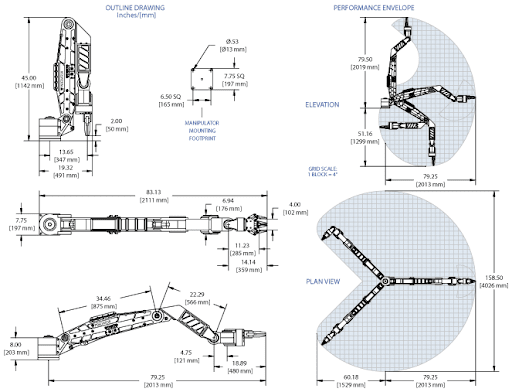
\includegraphics[width=.5\linewidth]{blueprint-arm} 
        %       \caption{DFT, Initial condition} 
        %     \end{minipage}
        %     \hfill
        %     \begin{minipage}[b]{0.5\linewidth}
        %       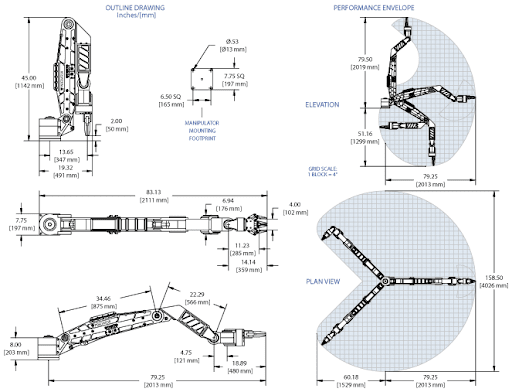
\includegraphics[width=.5\linewidth]{blueprint-arm} 
        %       \caption{DFT, rupture} 
        %     \end{minipage} 
        %   \end{figure}
    \end{columns}
    % \begin{itemize}
    %     \item Planejamento de trajetórias.
    %     \item Odometria visual.
    %     \item Manipuladores subaquáticos.
    %     \item Manipuladores autônomos.
    %     \item Manipuladores subaquáticos autônomos.
    %     \item Operação submarina autônoma.
    % \end{itemize}
    % \begin{block}
    %     {MANIPULADOR}{manipulador}
    % \end{block}

%*----------- notes
    \note[item]{Notes can help you to remember important information. Turn on the notes option.}
\end{frame}
%-
\begin{frame}[c]{Metodologia}
    %\transboxin[duration=1,direction=30]
    \centering
    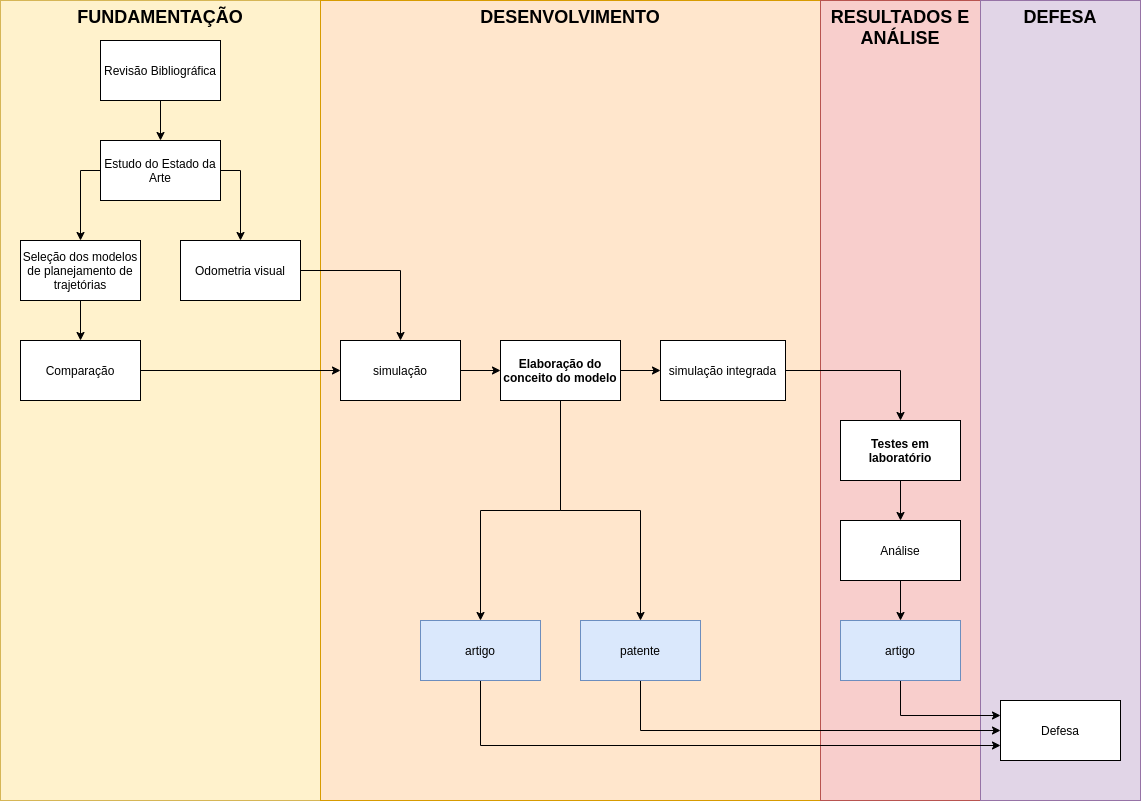
\includegraphics[width=0.7\textwidth]{metodologia11}
%*----------- notes
    \note[item]{Notes can help you to remember important information. Turn on the notes option.}
\end{frame}
%-
\begin{frame}[t]{Aspectos da Estatítisca na Metodologia}
    %\transboxin[duration=1,direction=30]

    % \centering
    % 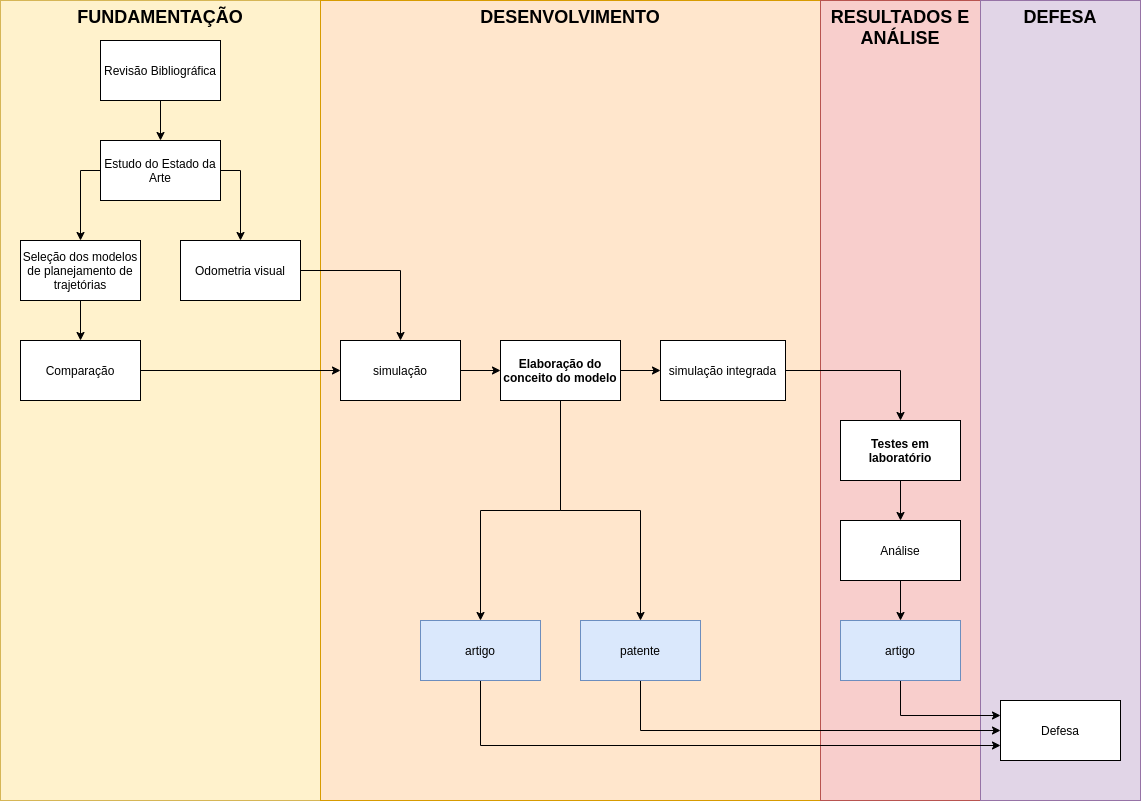
\includegraphics[width=0.3\textwidth]{metodologia11}

    No processo \textbf{Simulação} serão testados 
    \begin{itemize}
        \item os modelos de planejamento de trajetória selecionados na fase de \textbf{FUNDAMENTAÇÃO}; e
        \item os modelos de odometria visual.
    \end{itemize}
    Estes modelos ainda não foram definidos e serão testados de forma isolada. Está prevista uma \textit{Análise de Variância} dos erros comparativos entre o planejado e o executado de cada um dos modelos. 
    O tempo não será levado em consideração pelo fato de estar sendo usado o simulador GAZEBO\footnote{Simulador de robótica 3D de código aberto, integra o motor de física ODE, renderização OpenGL e código para simulação de sensores e controle de atuadores.}, o tempo referencial é baseado no tempo de uso dos processadores durante a simulação, dessa forma sendo consideração impreciso na sua marcação.

%*----------- notes
    \note[item]{Notes can help you to remember important information. Turn on the notes option.}
\end{frame}
%-
\begin{frame}[t]{Aspectos da Estatítisca na Metodologia}
    %\transboxin[duration=1,direction=30]

    % \centering
    % 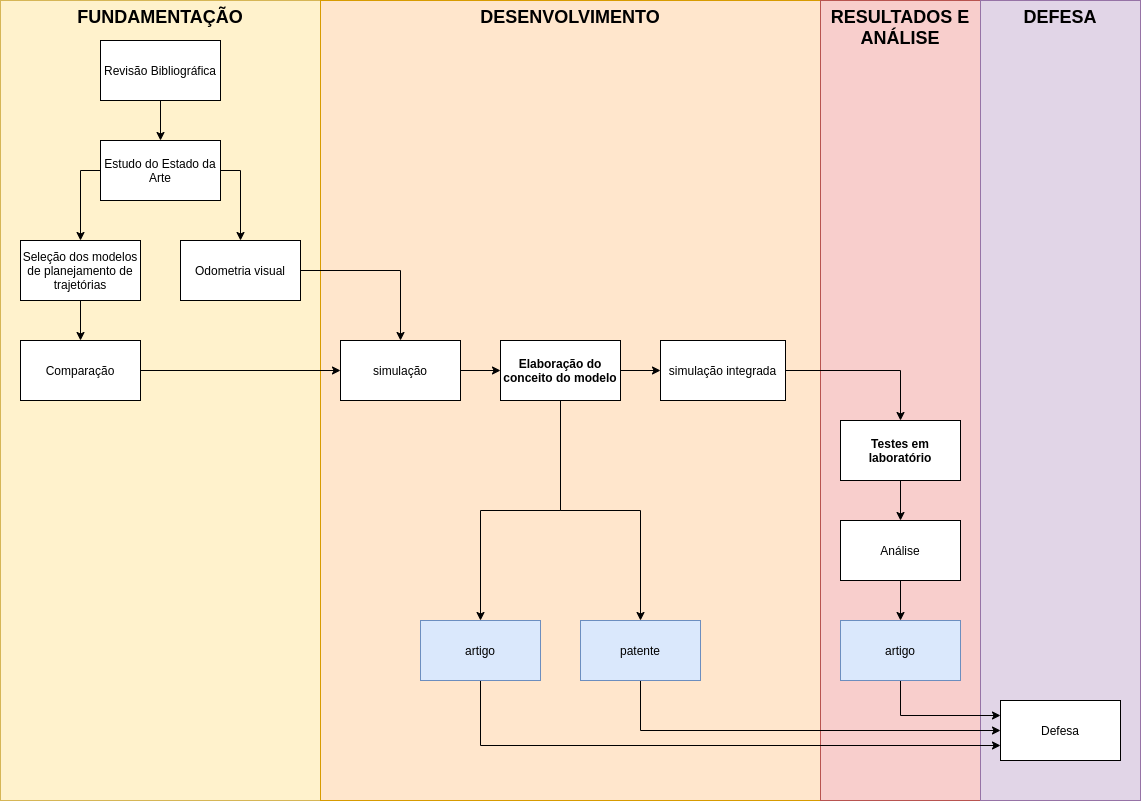
\includegraphics[width=0.3\textwidth]{metodologia11}

    No processo \textbf{Simulação Integrada} os modelos testados serão combinados com os modelos de planejamento e odometria, sendo agora acrescentado o modelo da tese em questão.
    Da mesma forma que o processo anterior, será utilizado uma \textit{Análise de Variância} para determinar o potencial do modelo sugerido frente a combinação dos outros modelos pré-definidos.
    \vspace*{0.2cm}

    Nesta etapa do \textbf{DESENVOLVIMENTO}, a estatística estará amparando estes dois processos da metodologia; o foco principal do uso da estatística estará fortemente sendo considerado na etapa de \textbf{RESULTADOS E ANAĹISE}.
    \vspace*{0.2cm}

    Vale ressaltar que não serão consideradas as váriáveis externas ao sistema: luminosidade, pressão e sujidade da água; ficando somente a perturbação utilizada tanto para a simulação como para os testes no laboratório.
%*----------- notes
    \note[item]{Notes can help you to remember important information. Turn on the notes option.}
\end{frame}
%-
\begin{frame}[t]{Aspectos da Estatítisca na Metodologia}
    %\transboxin[duration=1,direction=30]

    % \centering
    % 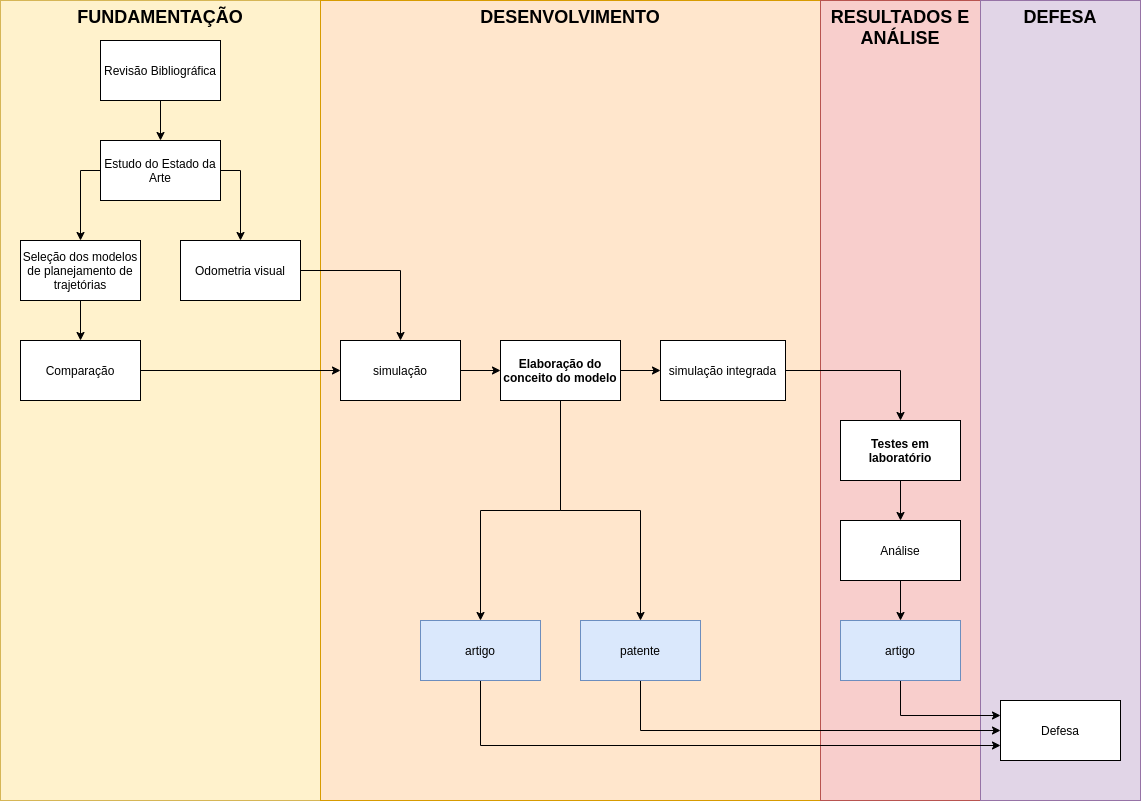
\includegraphics[width=0.3\textwidth]{metodologia11}

    Na etapa de \textbf{RESULTADOS E ANÁLISE}, dois processos são considerados:
    \begin{itemize}
        \item testes em laboratório; e 
        \item análise.
    \end{itemize}
    Estes testes serão realizados com o manipulador UR-5 integrado na plataforma móvel Warthog.

    \begin{columns}
        \column{.02\textwidth}
        \column{.45\textwidth}
            \centering
            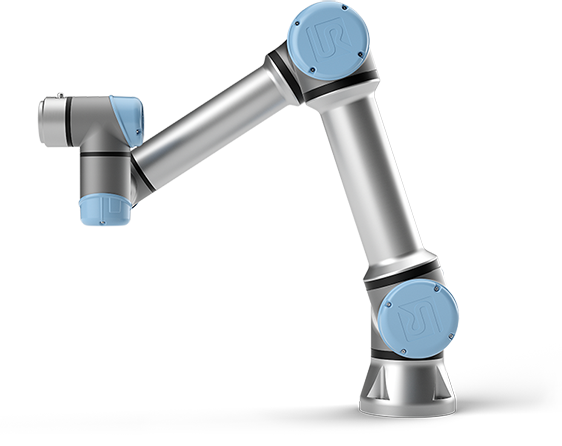
\includegraphics[width=.8\textwidth]{ur5e}
        \column{.45\textwidth}
            \centering
            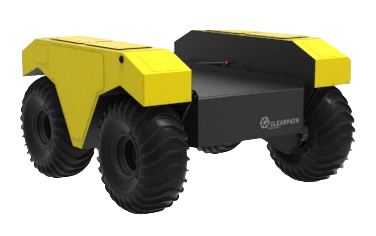
\includegraphics[width=1\textwidth]{warthog}
    \end{columns}

%*----------- notes
    \note[item]{Notes can help you to remember important information. Turn on the notes option.}
\end{frame}
%-
\begin{frame}[t, shrink=10]{Aspectos da Estatítisca na Metodologia}
    %\transboxin[duration=1,direction=30]

    Basicamente será realizado um \textit{Planejamento de Experimentos} tomando as variáveis independentes como: \textbf{modelo de planejamento}, \textbf{modelo de odometria}, \textbf{tipo de trajetória}, e \textbf{modo de perturbação}.
    \vspace*{0.2cm}

    Conforme apontado anteriormente os níveis desejados dos modelos ainda não foram definidos porém para o tipo de trajetória será planejado dois níveis: linear e circular; e para o modo de perturbação será considerado dois níveis de pertubação no qual caracterizará as correntes marítimas que causam perturbações nas trajetórias de manipuladores submarinos.

    \vspace*{0.2cm}
    Os resultados esperados serão o tempo de execução da trajetória e o erro comparativo; buscando entender a interação entre as várias independentes e as dependentes.

    \vspace*{0.2cm}
    Após a constatação da eficiência do modelo proposto, será realizado um último teste com o modelo buscando a Repetibilidade e Reprodutibilidade do modelo diante dos tipos de trajetórias propostas anteriormente, mostrando dessa forma uma certa aceitabilidade para as perturbações testadas.

%*----------- notes
    \note[item]{Notes can help you to remember important information. Turn on the notes option.}
\end{frame}
%-
% \begin{frame}[c]{Cronograma}
%     %\transboxin[duration=1,direction=30]
%     \centering
%     % \begin{columns}
%     %     \column{.05\textwidth}
%     %     \column{.95\textwidth}
%         % Please add the following required packages to your document preamble:
% % \usepackage[table,xcdraw]{xcolor}
% % If you use beamer only pass "xcolor=table" option, i.e. \documentclass[xcolor=table]{beamer}
% \begin{table}[]
%     \resizebox{\linewidth}{!}{
%     \begin{tabular}{llll|llllllllllll|llllllllllll}
%     \cline{3-28}
%      & \multicolumn{1}{l|}{} & \multicolumn{2}{c|}{2020} & \multicolumn{12}{c|}{2021} & \multicolumn{12}{c|}{2022} \\ \cline{3-28} 
%      & \multicolumn{1}{l|}{} & \multicolumn{1}{c}{J - N} & \multicolumn{1}{c|}{D} & \multicolumn{1}{c}{J} & \multicolumn{1}{c}{F} & \multicolumn{1}{c}{M} & \multicolumn{1}{c}{A} & \multicolumn{1}{c}{M} & \multicolumn{1}{c}{J} & \multicolumn{1}{c}{J} & \multicolumn{1}{c}{A} & \multicolumn{1}{c}{S} & \multicolumn{1}{c}{O} & \multicolumn{1}{c}{N} & \multicolumn{1}{c|}{D} & \multicolumn{1}{c}{J} & \multicolumn{1}{c}{F} & \multicolumn{1}{c}{M} & A & M & J & J & A & S & O & N & D \\ \hline
%      & \textbf{Disciplinas - cumprimento de créditos} & \textbf{\textgreater{}\textgreater{}\textgreater{}} & \textbf{\textgreater{}} & \textbf{\textgreater{}} & \textbf{\textgreater{}} & \textbf{\textgreater{}} & \textbf{\textgreater{}} & \textbf{\textgreater{}} &  &  &  &  &  &  &  &  &  &  &  &  &  &  &  &  &  &  &  \\ \hline
%      & \textbf{Fundamentação} &  & \textbf{\textgreater{}} & \textbf{\textgreater{}} & \textbf{\textgreater{}} & \textbf{\textgreater{}} & \textbf{\textgreater{}} & \textbf{\textgreater{}} & \textbf{\textgreater{}} &  &  &  &  &  &  &  &  &  &  &  &  &  &  &  &  &  &  \\ \hline
%     1 & Fazer revisão bibliográfica &  & \textgreater{} & \textgreater{} &  &  &  &  &  &  &  &  &  &  &  &  &  &  &  &  &  &  &  &  &  &  &  \\
%     2 & Elaborar estudo do estado da arte &  &  &  & \textgreater{} & \textgreater{} &  &  &  &  &  &  &  &  &  &  &  &  &  &  &  &  &  &  &  &  &  \\
%     3 & Comparar modelos pesquisados &  &  &  &  & \textgreater{} &  &  &  &  &  &  &  &  &  &  &  &  &  &  &  &  &  &  &  &  &  \\
%     4 & Estudar odometria visual &  &  &  &  & \textgreater{} & \textgreater{} &  &  &  &  &  &  &  &  &  &  &  &  &  &  &  &  &  &  &  &  \\
%     5 & {\color[HTML]{3166FF} \textit{Escrever parte.1 da tese (introdução, fundamentação e metodologia)}} &  &  &  & \textgreater{} & \textgreater{} & \textgreater{} & \textgreater{} & \textgreater{} &  &  &  &  &  &  &  &  &  &  &  &  &  &  &  &  &  &  \\
%     6 & {\color[HTML]{9A0000} Realizar qualificação} &  &  &  &  &  &  &  & \textgreater{} &  &  &  &  &  &  &  &  &  &  &  &  &  &  &  &  &  &  \\ \hline
%      & \textbf{Desenvolvimento} &  &  &  &  &  &  &  & \textbf{\textgreater{}} & \textbf{\textgreater{}} & \textbf{\textgreater{}} & \textbf{\textgreater{}} & \textbf{\textgreater{}} & \textbf{\textgreater{}} & \textbf{\textgreater{}} &  &  &  &  &  &  &  &  &  &  &  &  \\ \hline
%     1 & Realizar simulação dos modelos e odometria &  &  &  &  &  &  &  & \textgreater{} & \textgreater{} & \textgreater{} &  &  &  &  &  &  &  &  &  &  &  &  &  &  &  &  \\
%     2 & Elaborar conceito do novo modelo &  &  &  &  &  &  &  &  &  & \textgreater{} & \textgreater{} &  &  &  &  &  &  &  &  &  &  &  &  &  &  &  \\
%     3 & Realizar simulação integrada &  &  &  &  &  &  &  &  &  &  & \textgreater{} & \textgreater{} &  &  &  &  &  &  &  &  &  &  &  &  &  &  \\
%     4 & {\color[HTML]{3166FF} \textit{Escrever primeiro artigo}} &  &  &  &  &  &  &  &  &  &  &  & \textgreater{} & \textgreater{} & \textgreater{} &  &  &  &  &  &  &  &  &  &  &  &  \\
%     5 & {\color[HTML]{3166FF} \textit{Escrever patente}} &  &  &  &  &  &  &  &  &  &  &  & \textgreater{} & \textgreater{} & \textgreater{} &  &  &  &  &  &  &  &  &  &  &  &  \\ \hline
%      & \textbf{Resultados e análise} &  &  &  &  &  &  &  &  &  &  &  &  & \textbf{\textgreater{}} & \textbf{\textgreater{}} & \textbf{\textgreater{}} & \textbf{\textgreater{}} & \textbf{\textgreater{}} & \textbf{\textgreater{}} & \textbf{\textgreater{}} & \textbf{\textgreater{}} &  &  &  &  &  &  \\ \hline
%     1 & Realizar testes em laboratório &  &  &  &  &  &  &  &  &  &  &  &  & \textgreater{} & \textgreater{} & \textgreater{} & \textgreater{} &  &  &  &  &  &  &  &  &  &  \\
%     2 & Analisar os dados obtidos &  &  &  &  &  &  &  &  &  &  &  &  &  &  &  & \textgreater{} & \textgreater{} &  &  &  &  &  &  &  &  &  \\
%     3 & {\color[HTML]{3166FF} \textit{Escrever segundo artigo}} &  &  &  &  &  &  &  &  &  &  &  &  &  &  &  &  &  & \textgreater{} & \textgreater{} & \textgreater{} &  &  &  &  &  &  \\ \hline
%      & \textbf{Defesa} &  &  &  &  &  &  &  &  &  &  &  &  &  &  &  &  &  &  &  & \textbf{\textgreater{}} & \textbf{\textgreater{}} & \textbf{\textgreater{}} & \textbf{\textgreater{}} & \textbf{\textgreater{}} & \textbf{\textgreater{}} & \textbf{\textgreater{}} \\ \hline
%     1 & {\color[HTML]{3166FF} \textit{Escrever parte.2 da tese (Resultados e análise e conclusão)}} &  &  &  &  &  &  &  &  &  &  &  &  &  &  &  &  &  &  &  & \textgreater{} & \textgreater{} & \textgreater{} & \textgreater{} & \textgreater{} &  &  \\
%     2 & {\color[HTML]{9A0000} Realizar defesa perante a banca} &  &  &  &  &  &  &  &  &  &  &  &  &  &  &  &  &  &  &  &  &  &  &  &  & \textgreater{} & \textgreater{}
%     \end{tabular}
%     }
% \end{table}

%     % \end{columns}

% %*----------- notes
%     \note[item]{Notes can help you to remember important information. Turn on the notes option.}
% \end{frame}
%-
\begin{frame}[c]{Referências}
    %\transboxin[duration=1,direction=30]
    %\centering
    %\bibliographystyle{apalike}
%     \textcite{agostini2007}
%     \parencite{agostini2007}
%     \footcite{agostini2007}
%     \cite{agostini2007}\\
% começo
%     \bibentry{agostini2007}
    \begin{columns}
    \column{.01\textwidth}
    \column{.95\textwidth}
    \Wider{
   
    GUANGYI, Z. et al. Research on underwater safety inspection and operational robot motion control. In: IEEE. 2018 33rd Youth Academic Annual Conference of Chinese Association of Automation (YAC). [S.l.], 2018. p. 322–327.\\
    \vspace*{0.2cm}

    BRUNO, F. et al. Augmented reality visualization of scene depth for aiding rov pilots in underwater manipulation. Ocean Engineering, Elsevier, v. 168, p. 140–154, 2018.\\
    \vspace*{0.2cm}

    LEBORNE, F. et al. Dynamic modeling and identification of an heterogeneously actuated underwater manipulator arm. In: IEEE. 2018 IEEE International Conference on Robotics and Automation (ICRA). [S.l.], 2018. p. 1–9.\\
    \vspace*{0.2cm}

    BARBIERI, L. et al. Design, prototyping and testing of a modular small-sized underwater robotic arm controlled through a master-slave approach. Ocean Engineering, Elsevier, v. 158, p. 253–262, 2018.


    }
    \end{columns}
%*----------- notes
    \note[item]{Notes can help you to remember important information. Turn on the notes option.}
\end{frame}
%-
\begin{frame}[t]{Referências}
    %\transboxin[duration=1,direction=30]
    %\centering
    \begin{columns}
        \column{.01\textwidth}
        \column{.95\textwidth}
        \Wider{
       
        KURUMAYA, S. et al. A modular soft robotic wrist for underwater manipulation. Soft robotics, Mary Ann Liebert, Inc. 140 Huguenot Street, 3rd Floor New Rochelle, NY 10801 USA, v. 5, n. 4, p. 399–409, 2018.\\
        \vspace*{0.2cm}
    
        SIVČEV, S. et al. Underwater manipulators: A review. Ocean Engineering, Elsevier, v. 163, p. 431–450, 2018. \\
        \vspace*{0.2cm}
    
        SIVČEV, S. et al. Collision detection for underwater rov manipulator systems. Sensors, Multidisciplinary Digital Publishing Institute, v. 18, n. 4, p. 1117, 2018.
        }
        \end{columns}
    
    
    
    
    

%*----------- notes
    %\note[item]{Notes can help you to remember important information. Turn on the notes option.}
\end{frame}
%-